
% This LaTeX was auto-generated from MATLAB code.
% To make changes, update the MATLAB code and republish this document.

\documentclass{article}
\usepackage{graphicx}
\usepackage{color}

\sloppy
\definecolor{lightgray}{gray}{0.5}
\setlength{\parindent}{0pt}

\begin{document}

    
    
\subsection*{Contents}

\begin{itemize}
\setlength{\itemsep}{-1ex}
   \item original system
   \item observer design
   \item error signals
   \item plots
\end{itemize}
\begin{verbatim}
clear; clc;
\end{verbatim}


\subsection*{original system}

\begin{verbatim}
u = @(t) 0;
fx = @(t,x) [ x(2) ;...
            -x(2) - sin(x(1)) + u(t)];

tspan = [0 4];
y0 = [pi/3; 0];
[t,y] = ode45(@(t,y) fx(t,y),tspan,y0);
\end{verbatim}


\subsection*{observer design}

\begin{verbatim}
y_val = @(tt) interp1(t,y(:,1),tt,'spline');
beta = 5;
K = [beta; 1];
fo = @(t,x) fx(t,x) + K * (y_val(t) - x(1));

y0 = [-pi/6; -pi/10];
[to,yo] = ode45(@(t,y) fo(t,y),tspan,y0);
\end{verbatim}


\subsection*{error signals}

\begin{verbatim}
yoo = interp1(t,y,to,'spline');
err = (yo - yoo);
\end{verbatim}


\subsection*{plots}

\begin{verbatim}
figure(1); clf;
tiledlayout(3,2)

% nexttile([1 2]);
% plot(y(:,1),y(:,2)); grid off; box off;
% ylabel('$x_2$','Interpreter','latex');
% xlabel('$x_1$','Interpreter','latex');

ax(1) = nexttile([2 1]);
plot(t,rad2deg(y(:,1))); hold on
plot(to,rad2deg(yo(:,1))); grid off; box off;
ylabel('$x_1$ [$^\circ$]','Interpreter','latex');
xlabel('$t$ [s]','Interpreter','latex');

ax(2) = nexttile([2 1]);
plot(t,rad2deg(y(:,2))); hold on
plot(to,rad2deg(yo(:,2))); grid off; box off;
ylabel('$x_2$ [$^\circ$/s]','Interpreter','latex');
xlabel('$t$ [s]','Interpreter','latex');

ax(3) = nexttile();
plot(to,rad2deg(err(:,1))); box off
ylabel('$e_1$ [$^\circ$]','Interpreter','latex');
xlabel('$t$ [s]','Interpreter','latex');
yline(0,'--')

ax(4) = nexttile();
plot(to,rad2deg(err(:,2))); box off
ylabel('$e_2$ [$^\circ$/s]','Interpreter','latex');
xlabel('$t$ [s]','Interpreter','latex');
yline(0,'--')

linkaxes(ax,'x')

% Get latex font in ticks
h = findall(gcf,'Type','axes'); % An array if you have subplots
set(h, 'TickLabelInterpreter', 'latex')

textwidth = 13;
golden_ratio = (1 + sqrt(5)) / 2;
textheight = textwidth / golden_ratio;
figsize = [textwidth, textheight];

newcolors = ["#1f77b4" "#ff7f0e" "#2ca02c" "#d62728"];
colororder(newcolors)

% Set size and no crop
set(gcf, 'PaperUnits', 'centimeters', 'PaperSize', figsize);
set(gcf, 'PaperUnits', 'normalized', 'PaperPosition', [0, 0, 1, 1]);

print -dpdf ../doc/figures/ex2_6.pdf
\end{verbatim}

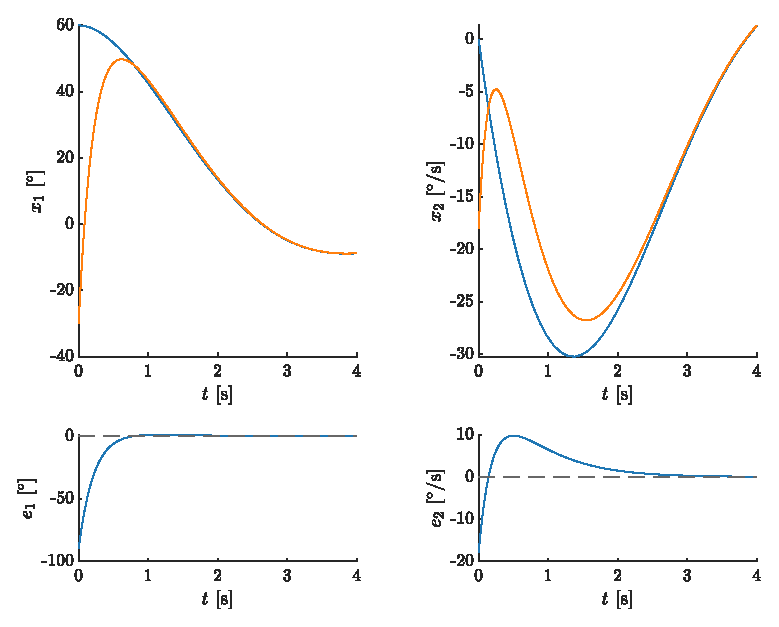
\includegraphics [width=4in]{Le2_6_01.eps}



\end{document}

